\documentclass[10pt]{article}
\usepackage{amsmath}
\usepackage{amsfonts}
\usepackage{pstricks,pst-eps}
\usepackage{tikz}
\pagestyle{empty}
\begin{document}
	\begin{TeXtoEPS}
		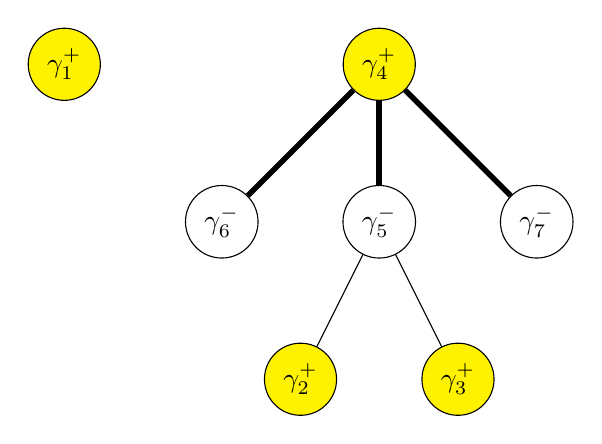
\begin{tikzpicture}
			\node[circle,draw,fill=yellow](n4) at (0,0)
			{$\gamma_4^+$};
			\node[circle,draw](n6) at (-2,-2) {$\gamma_6^-$};
			\node[circle,draw](n5) at (0,-2) {$\gamma_5^-$};
			\node[circle,draw](n7) at (2,-2) {$\gamma_7^-$};
			\node[circle,draw,fill=yellow](n2) at (-1,-4)
			{$\gamma_2^+$};
			\node[circle,draw,fill=yellow](n3) at (+1,-4)
			{$\gamma_3^+$};
			\node[circle,draw,fill=yellow](n1) at (-4,0)
			{$\gamma_1^+$};
			\draw[line width=2] (n4)--(n6);
			\draw[line width=2] (n4)--(n5);
			\draw[line width=2] (n4)--(n7);
			\draw (n5)--(n2);
			\draw (n5)--(n3);
		\end{tikzpicture}
	\end{TeXtoEPS}
\end{document}